\begin{figure*}[]
	\sidesubfloat[First subfigure]{%
	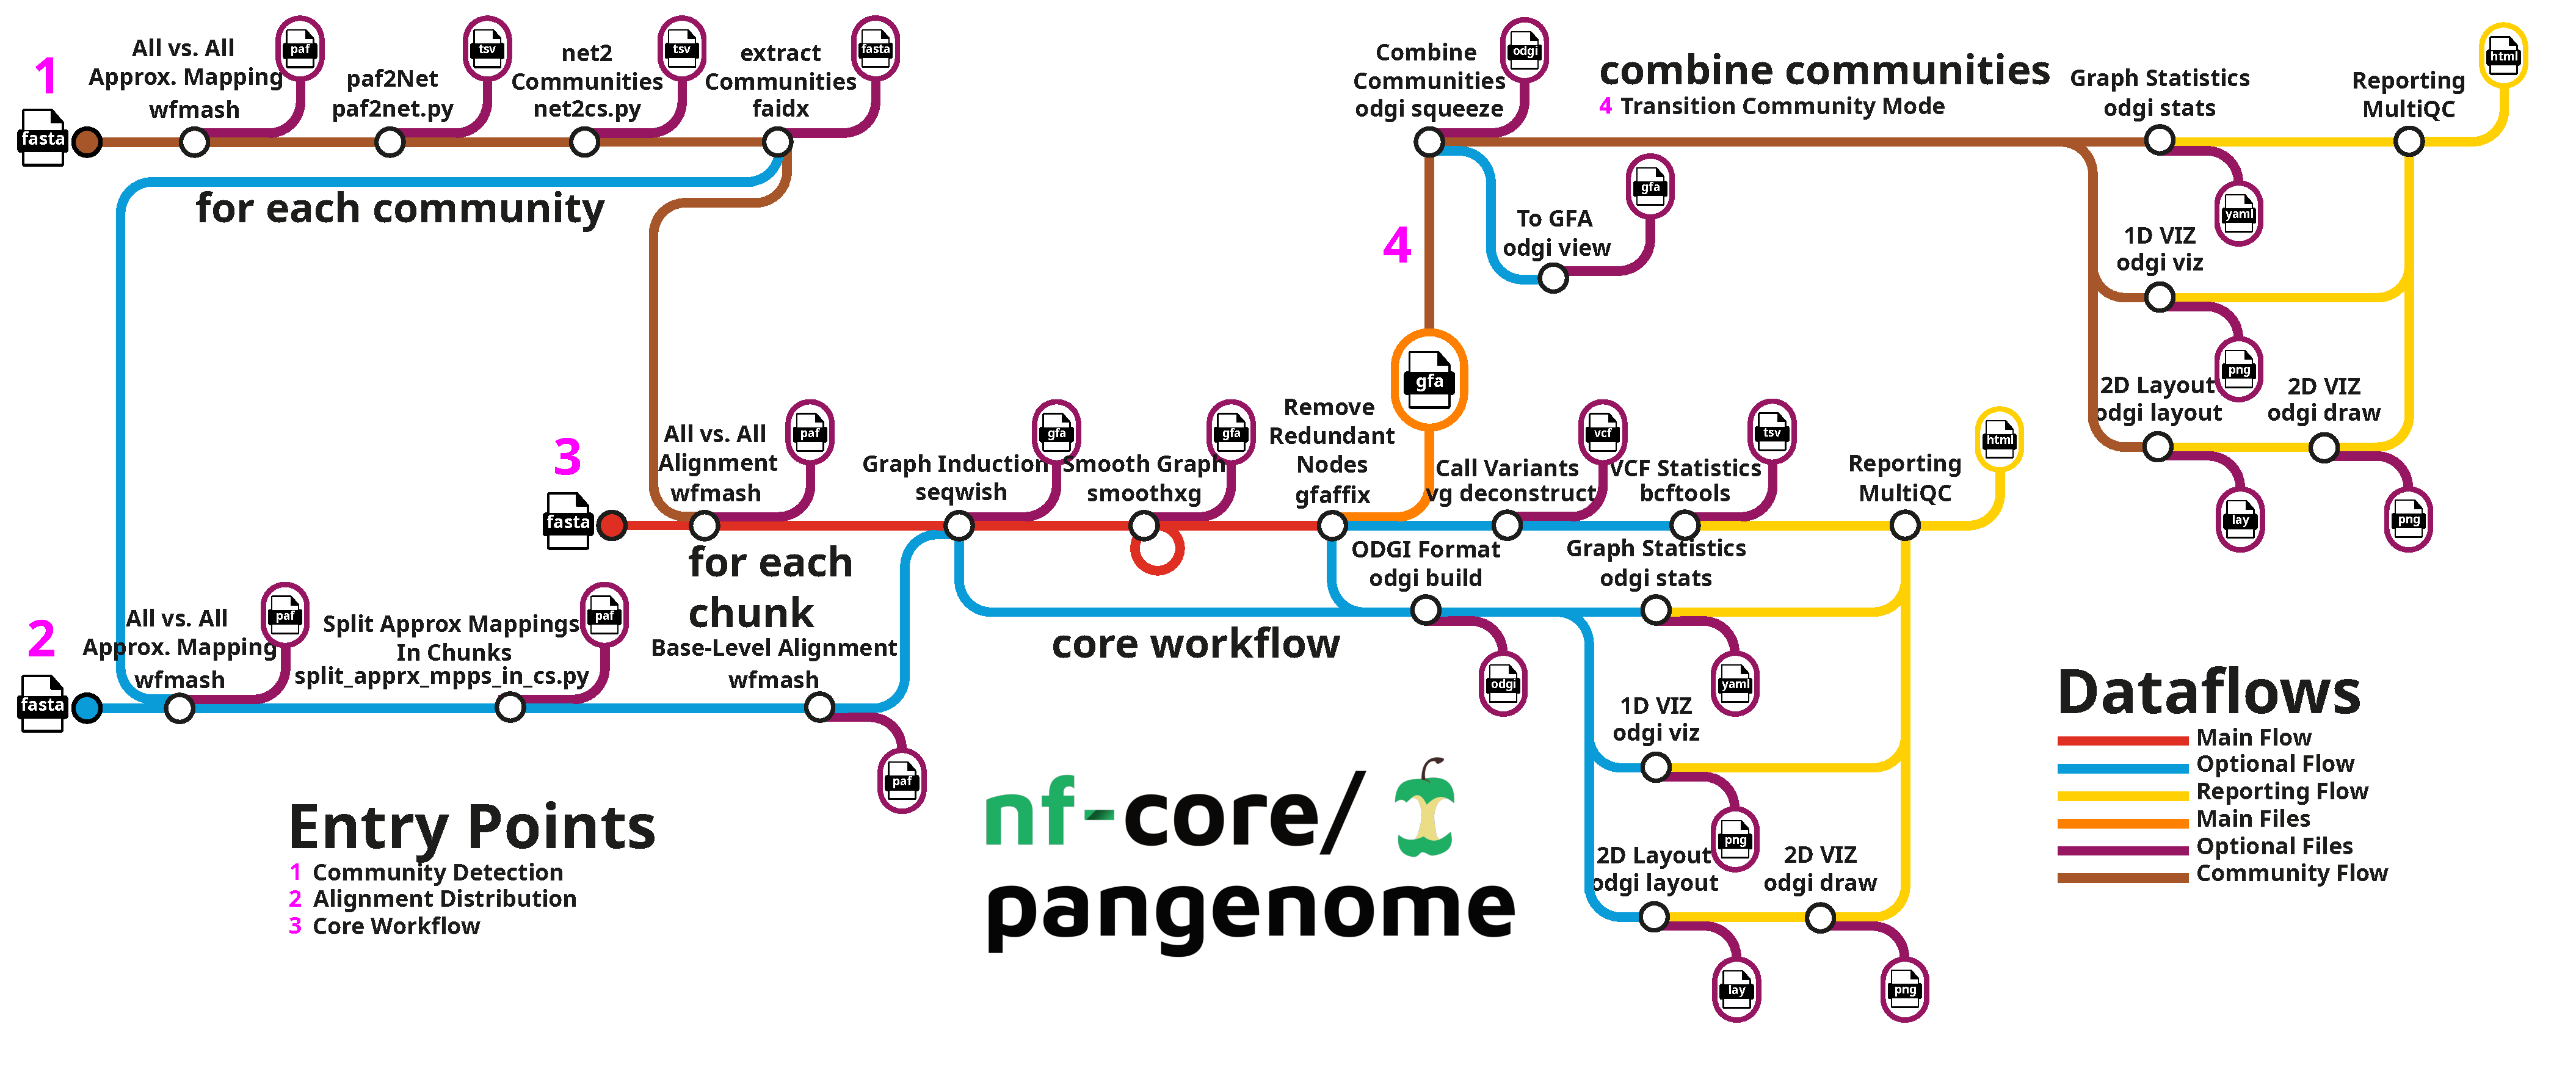
\includegraphics[width=\textwidth]{fig/pangenome_workflow.pdf}
	\label{fig:workflow}
	}
	\vspace{-0.3cm}
	\hfill
	\sidesubfloat[Second subfigure]{%
	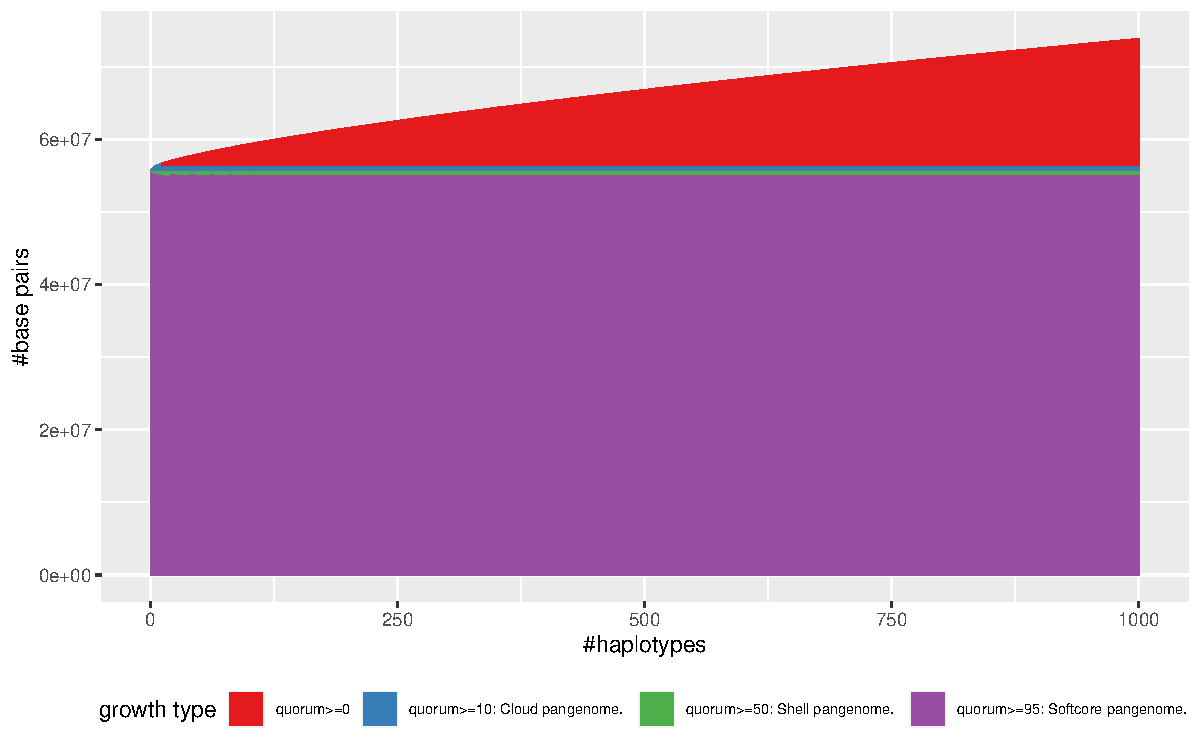
\includegraphics[width=0.45\textwidth]{fig/chr19_histgrowth.pdf}
	\label{fig:hist_chr19}
	}
	\sidesubfloat[Second subfigure]{%
	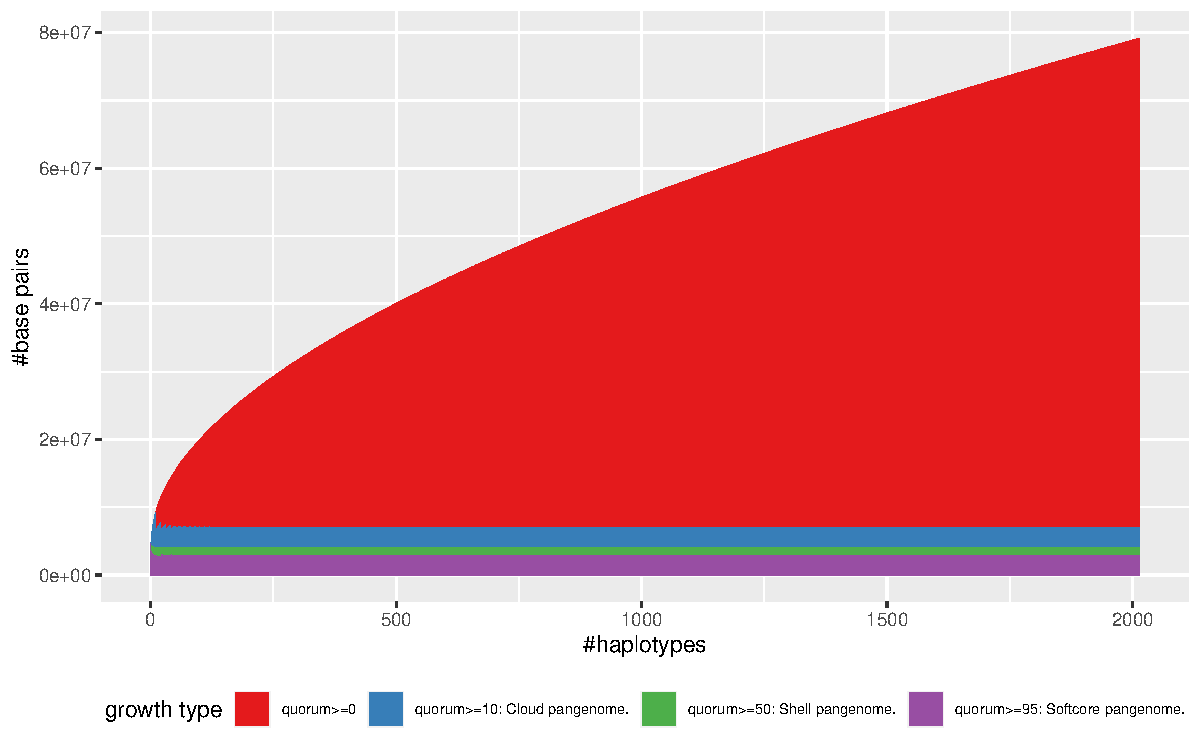
\includegraphics[width=0.45\textwidth]{fig/ecoli2013_histgrowth.pdf}
	\label{fig:hist_ecoli}
	}
	%\sidesubfloat[Second subfigure]{%
	%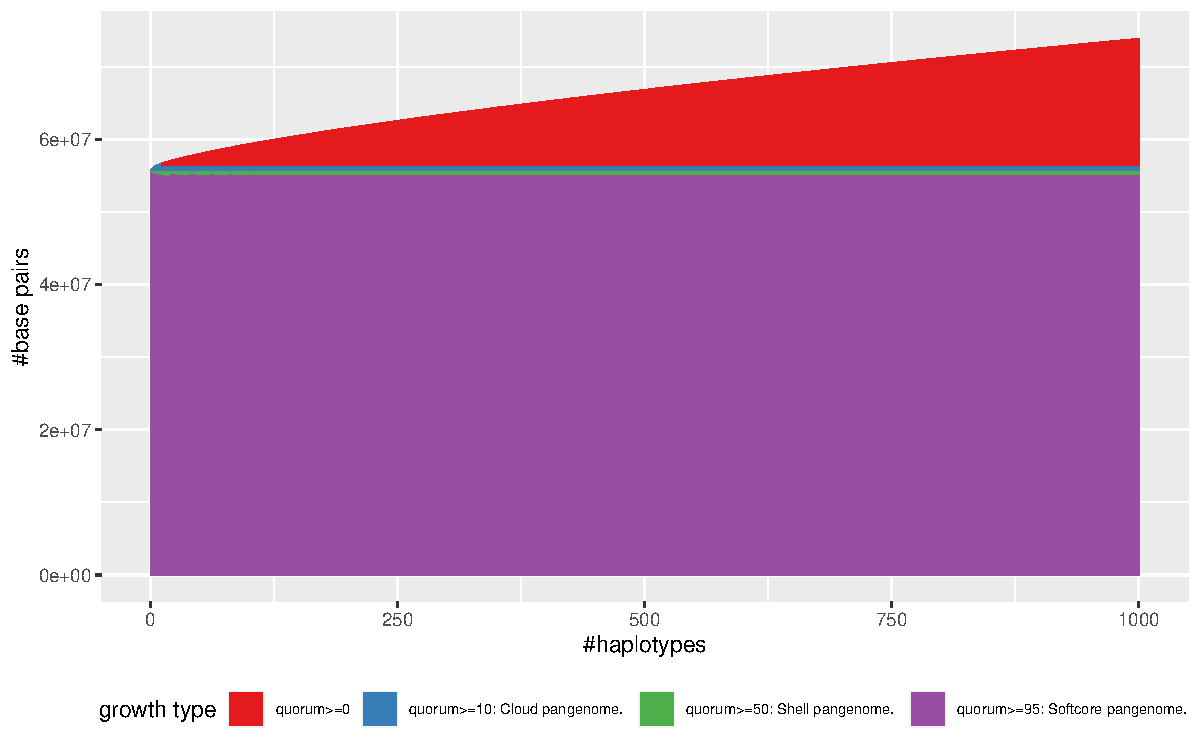
\includegraphics[width=0.3\textwidth]{fig/chr19_histgrowth.pdf}
	%\label{fig:hist_ecoli}
	%}
	\vspace{-0.25cm}
	\caption{\textbf{(a)} Schematic representation of the nf-core/pangenome workflow processes and detailed analysis steps. The input consists of one FASTA file containing all sequences. The pipeline comes with 3 major entry points: \red{(1) Community detection, which identifies clusters of related sequences or regions in the pangenome graph to reveal biologically significant patterns like conserved or divergent areas across genomes~(Supplementary \ref{community}), (2) alignment distribution, and (3)  core workflow.} Optional community detection (1) is performed on the input sequences. If selected, the heavy all-to-all baise-pair level alignments (2) can be split into problems of equal size. nf-core/pangenome’s core workflow (3) is a direct mirror of PGGB. If running in community mode, all communal graphs are combined into one (4) and the subsequent quality control subworkflow is executed. The output is a pangenome graph in GFA format. \textbf{(b) + (c)} Pangenome growth curves of the built pangenome graphs. Growth type is defined as the minimum fraction of haplotypes that must share a graph feature after each time a haplotype is added to the growth histograph. $quorum>=0$: All sequences without any filtering are considered. $quorum>=10$: Sequences traversed by at least 10\% of the haplotypes. $quorum>=50$: Sequences traversed by at least 50\% of haplotypes. $quorum>=95$: Sequences traversed by 95\% of haplotypes. \textbf{(b)} Pangenome growth curve of the chromosome 19 pangenome graph of 1000 haplotypes. \textbf{(c)} Pangenome growth curve of the \textit{E. coli} pangenome graph of 2013 haplotypes.
	}
	\label{fig:panel}
\end{figure*}
\vspace{-0.4cm}